\section{Tamtam Listens}
\label{sec:tamtam-listens}

La aplicación desarrollada, denominada \emph{Tamtam Listens}, es el resultado de la combinación
de las tecnolog\'ias mencionadas anteriormente.

El reconocimiento de los comandos de voz se implement\'o como un servicio de \emph{dbus}\cite{Dbus2013}, que es
un mecanismo para comunicaci\'on entre procesos de linux. Por lo tanto, el servicio puede ser utilizado
no solo por \emph{Tamtam Listens} si no por cualquier aplicaci\'on de linux. 

\emph{Pocketsphinx} requiere de un modelo ac\'ustico y un modelo de lenguaje para realizar
el reconocimiento de comandos. Para el modelo ac\'ustico se utiliz\'o el prove\'ido por el proyecto \emph{Voxforge}
\cite{Voxforge}, que es un proyecto que busca proveer modelos ac\'usticos para motores de reconocimientos
de c\'odigo abierto. Para el modelo de lenguaje se defini\'o una gram\'atica JSGF\cite{JSGF2000}, que permiti\'o definir los
comandos soportados por la aplicaci\'on de una manera sencilla. A continuaci\'on se puede observar la gram\'atica utilizada
para definir los comandos soportados por \emph{Tamtam Listens} 


\lstset{
  basicstyle=\scriptsize,        % the size of the fonts that are used for the code
  breakatwhitespace=false,         % sets if automatic breaks should only happen at whitespace
  frame=single,                    % adds a frame around the code
  language=Octave,                 % the language of the code
  numbersep=5pt,                   % how far the line-numbers are from the code
  showstringspaces=false,          % underline spaces within strings only
  stepnumber=2,                    % the step between two line-numbers. If it's 1, each line will be numbered
  tabsize=2                       % sets default tabsize to 2 spaces
}

\begin{figure}[H]
\begin{lstlisting}
#JSGF V1.0;
grammar tamtam;

public <tamtam-listens> = <comando> | <pagina> | <pista-a>  | <pista-b>  | 
                          <seleccionar-compas> | <crear-nota> | <seleccionar-nota> | 
                          <duplicar-nota> | <borrar-nota> | <volumen> | <tempo> | 
                          <configurar-nota> | <loop>;

<comando> = REPRODUCIR MUSICA | PAUSAR MUSICA | PARAR MUSICA | GENERAR MUSICA | 
            CREAR NUEVA MUSICA | EXPORTAR MUSICA | SALIR DE TAMTAM;
<pagina> = ( CREAR NUEVA | DUPLICAR | LIMPIAR ) PARTITURA | PARTITURA <orden>;
<pista-a> = PISTA <numero> | DUPLICAR PISTA <numero> EN PISTA <numero>;
<pista-b> = [<instrumento> EN | REPRODUCIR | SILENCIAR | LIMPIAR | HABILITAR | 
             <volumen> DE] PISTA <numero>;
<instrumento> = ( <percusion> | <viento> | <cuerda> | <drum> | <teclado> );
<seleccionar-compas> = COMPAS <compas>;
<crear-nota> = CREAR NOTA <nota>;

<orden> = ( ANTERIOR | SIGUIENTE );
<numero> = ( UNO | DOS | TRES | CUATRO | CINCO );
<volumen> = ( AUMENTAR | DISMINUIR ) VOLUMEN;
<tempo> = ( AUMENTAR | DISMINUIR ) TEMPO;

<seleccionar-nota> = TIEMPO <nro-nota>;
<configurar-nota> = ( DURACION | INICIO EN TIEMPO ) <nro-nota>;


<duplicar-pista> = DUPLICAR EN <numero>;
<duplicar-nota> = DUPLICAR EN PISTA <numero> COMPAS <compas>;

<borrar-nota> = ELIMINAR NOTA;

<compas> = ( UNO | DOS | TRES | CUATRO );
<nota> = ( DO | RE | MI | FA | SOL | LA | SI ) [ GRAVE ] | DO AGUDO;
<nro-nota> = UNO | DOS | TRES | CUATRO | CINCO | SEIS | SIETE | OCHO | NUEVE | 
             DIEZ | ONCE | DOCE;

<percusion> = PERCUSION | TRIANGULO | CAMPANA;
<drum> = BATERIA | MADAL;
<viento> = VIENTO | FLAUTA | CLARINETE;
<cuerda> = CUERDA | GUITARRA ELECTRICA | GUITARRA ACUSTICA | BAJO;
<teclado> = TECLADO | PIANO | PIANO ELECTRICO | CLAVINET;

<loop> = (BASURA)+;
\end{lstlisting}
\caption{Gram\'atica utilizada en \emph{Tamtam Listens}}
\end{figure}

Por ejemplo, la representaci\'on en forma de grafo de la regla \emph{<crear-nota>} ser\'ia la que se
observa en la Figura~\ref{figure:cmd-nota}, donde un ejemplo de comando soportado es ``\emph{crear nota do}''

\begin{figure}[H]
\centering
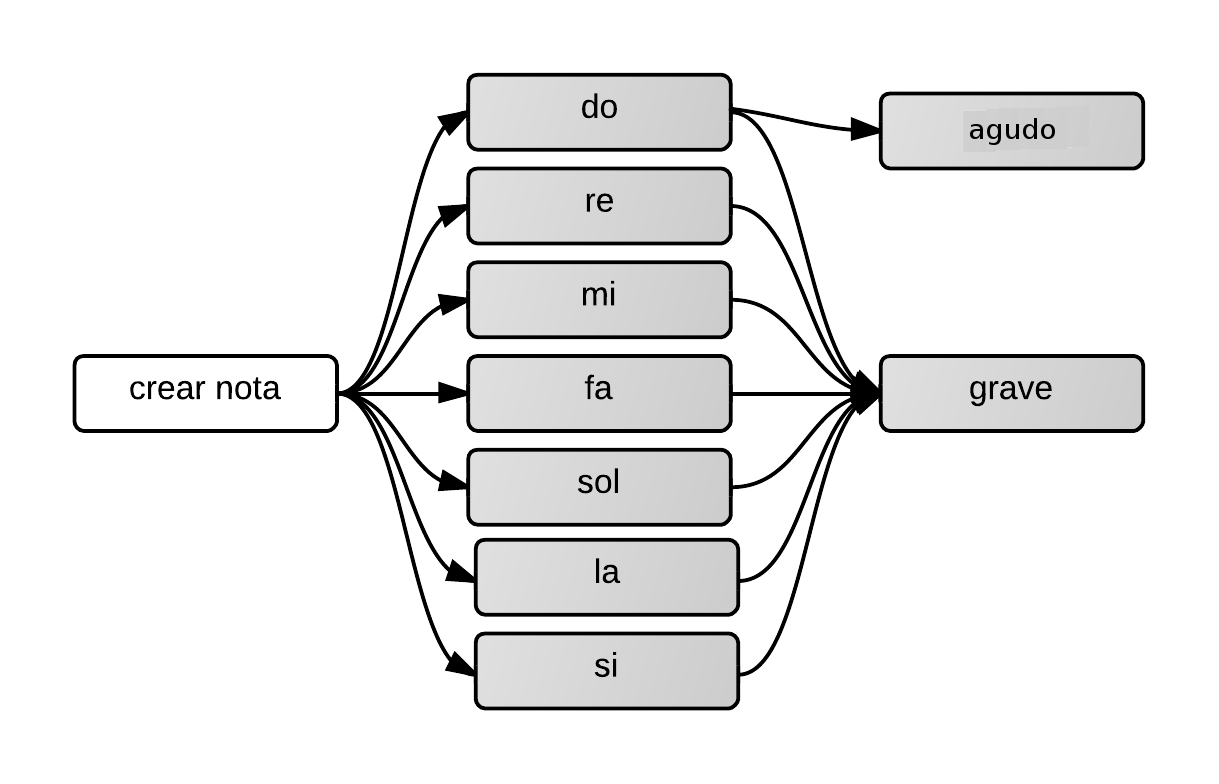
\includegraphics[width=0.5\textwidth]{./graphics/cmd-crear-nota.png}
\caption{Representaci\'on en forma de grafo de la regla \emph{<crear-nota>}}
\label{figure:cmd-nota}
\end{figure}


Otro elemento requerido por \emph{Pocketsphinx} es el diccionario, que permite mapear
palabras a secuencia de fonemas. En la siguiente figura se muestra un fragmento del diccionario
utilizado por la aplicaci\'on.

\begin{figure}[H]
\begin{lstlisting}
REPRODUCIR RR E P R O D U S I R
PAUSAR P A U S A R
PARAR  P A R A R
GENERAR  J E N E R A R
P\'aGINA P A J I N A
PARTITURA P A R T I T U R A
SIGUIENTE S I G I E N T E
ANTERIOR A N T E R I O R
\end{lstlisting}
\caption{Gram\'atica utilizada en \emph{Tamtam Listens}}
\end{figure}

La combinaci\'on de estos componentes es lo que permite a \emph{Pocketsphinx} realizar el
reconocimiento de los comandos de voz.
